\documentclass[conference]{IEEEtran}

\IEEEoverridecommandlockouts
\newcommand{\funding}{%
  This work is partially supported by EPSRC grant EP/G015740/1 (BIMPA); the European Union under grant nos. ERC-320689 (BIMPC), FP7-287701 (BrainScales-Extension), and FP7-604102 (HBP); and by the U.S.\ Office of Naval Research.
}

\title{An efficient SpiNNaker implementation of the Neural~Engineering~Framework}
\author{%
  \IEEEauthorblockN{Andrew~Mundy and Jamie~Knight}
  \IEEEauthorblockA{School of Computer Science,\\
                    University of Manchester,\\
                    Oxford Road, Manchester,\\
                    M13 9PL, UK\\
                    Email: andrew.mundy@ieee.org}
  \and
  \IEEEauthorblockN{Terrence~C.~Stewart}
  \IEEEauthorblockA{Centre for Theoretical Neuroscience,\\
                    University of Waterloo,\\
                    Waterloo, ON,\\
                    Canada N2L 3G1\\
                    Email: tcstewar@uwaterloo.ca}
  \and
  \IEEEauthorblockN{Steve~Furber}
  \IEEEauthorblockA{School of Computer Science,\\
                    University of Manchester,\\
                    Oxford Road, Manchester,\\
                    M13 9PL, UK\\
                    Email: steve.furber@manchester.ac.uk}
  \thanks{\funding}
}

%% Utilities
\usepackage{booktabs}  %% Pleasant tables
\usepackage[binary-units]{siunitx}
\usepackage[caption=false, font=footnotesize]{subfig}
\usepackage{graphicx}
\usepackage[mode=buildmissing]{standalone}

%% Source highlighting
\usepackage{listings}
\lstset{
  language=Python,
  morekeywords={with,as},
  columns=flexible,
  gobble=2,
  basicstyle=\footnotesize,
  xleftmargin=1em,
}

%% Maths
\usepackage{amsmath}
\usepackage{amssymb}
\renewcommand{\vec}{\mathbf}  % Bold vectors
\newcommand{\semanticpointer}{\textbf}
\newcommand{\msemanticpointer}[1]{\mbox{\semanticpointer{#1}}}

%% Bibliographies
\usepackage[backend=bibtex, style=ieee, doi=false, url=false, maxbibnames=7]{biblatex}
\bibliography{paper}
\usepackage{xcolor}

\begin{document}
  \maketitle

  \begin{abstract}
The Neural Engineering Framework (NEF) is an hypothesis about how complex neural systems may be constructed and has recently been used to build the world's first functional brain model, Spaun.
While the NEF simplifies the design of neural networks, simulation using standard computer hardware is still computationally expensive -- often running far slower than biological real-time and scaling very poorly: problems the SpiNNaker neuromorphic simulator was designed to solve.
In this paper we (1) argue that employing the same model of computation used for simulating general purpose spiking neural networks on SpiNNaker for NEF models results in sub-optimal use of the architecture, and (2) provide and evaluate an alternative simulation scheme which overcomes the memory and compute challenges posed by the NEF.
This proposed method uses factored weight matrices rather than the full weight matrix to reduce memory usage.
Memory usage reductions of the order of~90\% are possible and in some cases it is possible to simulate 2000 neurons on a processing core, double the SpiNNaker architectural target.
  \end{abstract}

  \section{Introduction}

For a given power budget, two factors limit the simulation of neural networks on any computing platform: scale and time. Theoretically, any scale of network may be simulated but as scale increases simulation time follows.
Conversely, if the simulation time is limited (for example, if biological real-time is necessary) then only a limited scale of network may be simulated.
Specialised \textit{neuromorphic} hardware tries to avoid these constraints by parallelising and distributing computational effort and relying on dense interconnection of the computing elements.
The SpiNNaker platform \parencite{Furber2014} is one of a range of neuromorphic simulators (including Neurogrid \parencite{Benjamin2014}, BrainScaleS \parencite{Schemmel2010} and TrueNorth \parencite{Merolla2014}) which should benefit researchers of large-scale neural models.

The Neural Engineering Framework (NEF) \parencite{Eliasmith2004} is a hypothesis about how neurons may be used to encode abstract mathematical constructs,such as scalars and vectors, that we often used to model the real world.
Its successes so far include the Spaun model of cognition \parencite{Eliasmith2012} and a spiking neural network that encodes and decodes the main lexical relations in WordNet \parencite{Crawford2013}.
As with all neural systems, the NEF has proven costly to simulate: the Spaun model typically required \SI{2.5}{\hour} of compute time for \SI{1}{\second} of simulation \parencite[\S V]{Stewart2014}.
Two aspects of NEF networks that make them particularly costly to simulate are the high firing rates of individual neurons (often up to \SI{400}{\hertz}) and the dense synaptic matrices used to connect neuronal populations.
The former presents a significant communication cost to any specialised neuromorphic hardware and the latter requires that large amounts of memory be used to represent the neural network with all the associated costs of transferring large blocks of data that implies.

  In this paper we:
  \begin{enumerate}
    \item Argue that due to the properties of the NEF, the existing solutions and algorithms used to simulate neural networks on SpiNNaker will not scale satisfactorily to large-scale models such as Spaun.
    \item Detail a method by which features of the NEF may be used to reduce the memory and compute costs associated with its simulation.
  \end{enumerate}

We hope to use the result to run the full Spaun model in biological real-time.

  \section{Background}

In this section we briefly discuss the SpiNNaker platform and how neural networks are currently simulated on it before introducing the Neural Engineering Framework (NEF) and discussing how models built with it may act to stress SpiNNaker in various ways.

  \subsection{The SpiNNaker platform}

The SpiNNaker platform is a massively parallel architecture designed to simulate neural networks.
A SpiNNaker machine is constructed from a number of SpiNNaker chips, each connected to their six immediate neighbours using a chip-level interconnection network with a toroidal, triangular mesh topology.
Each SpiNNaker chip contains 18 ARM processing cores connected, via a network-on-chip, to each other and the external network through a multicast router.
Each core has two small tightly-coupled memories: \SI{32}{\kibi\byte} for instructions and \SI{64}{\kibi\byte} for data; and shares \SI{128}{\mebi\byte} of off-chip SDRAM with the other cores on the SpiNNaker chip.

SpiNNaker is an event-driven, message-passing computing architecture.
The software running on a core may transmit packets to other processing cores to indicate the occurrence of events or to share data.
A packet consists of a \SI{32}{\bit} key, used to direct the packet around the network and, optionally, a \SI{32}{\bit} data payload.
When a packet reaches a router, its key is inspected to determine which (if any) of the 18 processors and six external links attached to the router it should be forwarded to.
On receipt of a packet, a core executes a \textit{callback} function which may inspect the packet and schedule further execution as required.

  \subsection{Simulating neural nets on SpiNNaker}
  \label{sec:background/nn}

When simulating neural nets on a SpiNNaker machine each core is responsible for simulating a number of point neurons (in the order of a few hundred).
When one of these neuron spikes, it transmits a packet whose key uniquely identifies the neuron (for this it requires no payload).
This ``spike'' packet is then routed across the network fabric to the processing cores responsible for simulating each of the neurons that are connected to the firing neuron.
On receipt of a ``spike'' packet a core retrieves the row of the connectivity matrix associated with the firing neuron from SDRAM.
Each of these rows describes the synaptic weights and delays associated with the connections between the firing neuron and those simulated on the core.
Once a row is retrieved the weights are inserted into an input ring-buffer where they remain until the synaptic delay has elapsed and they are applied to the neuronal input current.

Using this system there are two primary constraints on the number of neurons that may be simulated on a single processing core:

  \begin{enumerate}
    \item The amount of memory required to store the synaptic weight matrices must fit within the space available to the core.
      This is \SI{8}{\mebi\byte} as each core is allocated $\frac{1}{16}$ of the \SI{128}{\mebi\byte} SDRAM.
    \item As the majority of processing time is spent in the synaptic processing pipeline, there must be sufficient time for the core to process all incoming `spike' packets; and retrieve and process the synaptic rows during one simulation time-step (see \parencite{Sharp2013}).
This time is a function of both the number of spikes received per time-step and the density of the synaptic matrix.
\textcite[\S III.C]{Sharp2013} indicate that at most there may be \num{5000} synaptic events per millisecond when running at biological real-time, where a single synaptic event indicates one spike being passed through a single synapse to a neuron on the receiving core.
  \end{enumerate}

These constraints may be met by either allocating fewer neurons to each processing core or by increasing the processing time used for each simulation time-step.
Hard time constraints are necessary when SpiNNaker is required to run in biological real-time, as it is in experiments with other neuromorphic hardware.
Processor constraints are present for those with access to only small SpiNNaker machines such as those mounted in mobile robots.

It should be noted that time is also a factor \textit{prior} to the start of any simulation.
All data required by the SpiNNaker machine during simulation must be transmitted to it through an ethernet interface, meaning that if more data is required on the machine, more time is required to prepare it for simulation.
\textcite{Sharp2013} note that this preparation time can be in the order of several minutes  -- something that is undesirable if a real-time simulator is desired.

  \subsection{The Neural Engineering Framework}
  \label{sec:background/nef}

The Neural Engineering Framework (NEF) extends the concept of ``preferred-direction vectors'' \parencite{Georgopoulos1986} to all neural populations.
Each population represents a vector within a particular space, within which, the firing rate of each neuron reflects the similarity of the represented vector to the neurons ``encoding'' vector.
Using the notation of \textcite{Stewart2014} this ``encoding'' of a variable in vector form into a neuronal response may be expressed as:

\begin{equation}
  \delta_{i}\left(\vec{x}\right) = G_{i}\left[ \alpha_i \vec{e}_i \cdot \vec{x} + J^{bias}_i \right]
  \label{eq:encoding}
\end{equation}

Which states that the firing response of neuron $i$ ($\delta_i$) to the represented value ($\vec{x}$) is the response of the neuron model ($G_{i}$) to an input consisting of a randomly selected gain term ($\alpha_i$), the encoding vector for the neuron ($\vec{e}_i$) and a fixed bias current ($J^{bias}_i$).
Correspondingly, ``decoding'' allows a transformation from the spiking actions of neurons into the domain of vectors.
Again using the notation of \textcite{Stewart2014} we can express this decoding process as:

\begin{equation}
  \vec{\hat{x}} = \sum\limits_{i=1}^{N} a_i(\vec{x})\vec{d}_i  \label{eq:decoding}
\end{equation}

Where the estimate of the original represented value ($\vec{\hat{x}}$) is the sum of the spiking activity of each neuron ($a_i$) multiplied by the linear decoder for the neuron ($\vec{d}_i$).
The decoding vectors may be selected to compute a function of the value represented by the population.
\figurename~\ref{fig:background/nef-1} illustrates the encoding of a two-dimensional value using four neurons -- the role of the encoding vectors can be seen in that each neuron becomes active for only a small range of the input space.

  \begin{figure}[!t]
    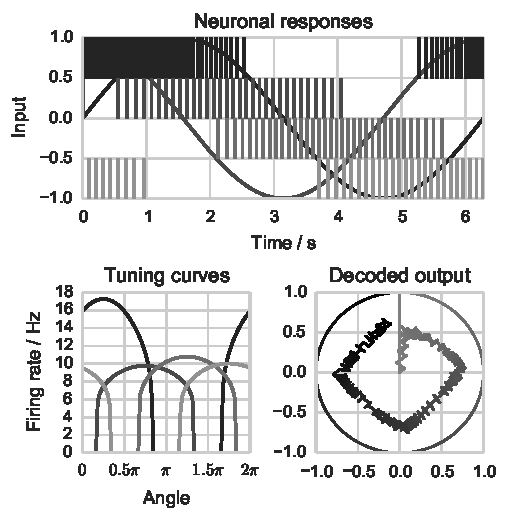
\includegraphics{figures/nef-1}
    \caption{%
      Representing a 2-dimensional value using four neurons. The input values and spiking responses of the neurons are shown in the top plot.
      The bottom left-hand plot shows how the firing responses vary with the angle of the 2-D input vector (tuning curves) and the bottom right-hand plot shows a decoding of the population's representation along with the input value.}
    \label{fig:background/nef-1}
  \end{figure}

%% Synaptic filtering
For a connection between a pair of populations, a (dense) synaptic weight matrix can be calculated by computing the matrix product of the decoders of the pre-synaptic population and the encoders of the post-synaptic population \parencite{Stewart2014}:

\begin{equation}
  \omega_{ij} = \alpha_j \vec{d_i}\vec{e_j}  \label{eq:weights}
\end{equation}

With $i$ indexing neurons in the pre-synaptic population and $j$ those in the post-synaptic population.

An illustrative model that we will use later in this paper is the \textit{communication channel}.
  A communication channel consists of two populations connected with the synaptic weights chosen such that the second ensemble will represent the same value as the first ensemble.
  The concept is illustrated in \figurename~\ref{fig:background/comms-channel}.

  \begin{figure}
    \centering
    \includestandalone[scale=0.75]{figures/comms_channel_map}
    \caption{A NEF communication channel consisting of two populations of neurons and a connection.
    The diagram indicates how the abstract communication channel might be instantiated on a simplified representation of the SpiNNaker architecture:
    Population $A$ is split between processing two cores, consequently two streams of multicast packets allow simulation of the communication channel.
    }
    \label{fig:background/comms-channel}
  \end{figure}
  
  \subsection{Assessing the Neural Engineering Framework (NEF)}
  \label{sec:background/assessing}

It is entirely possible to translate models built using NEF principles into populations of point neurons connected with dense synaptic weight matrices.
These networks could then, in theory, be simulated using the standard SpiNNaker spiking neural network simulator described in \S\ref{sec:background/nn}.
In this section we show that, based on parameters used in the Spaun functional brain model, this approach would result in sub-optimal usage of a SpiNNaker machine, given the constraints outlined in \S\ref{sec:background/nn}.

The Spaun model is built using the Semantic Pointer Architecture (SPA) \parencite{eliasmith2013build} which uses randomly chosen unit vectors to represent basic concepts.
These concepts can then be combined into symbol structures using addition~($+$) and circular convolution~($\circledast$) operators, both of which can be evaluated using the principles of the NEF.
The circular-convolution operator is non-linear and, Eliasmith \parencite{eliasmith2013build} demonstrates, require around 70 neurons per dimension to calculate accurately.

For example, using the basic concepts (\semanticpointer{MOUSE}, \semanticpointer{CHEESE}, \semanticpointer{SUBJECT}, \semanticpointer{OBJECT}, \semanticpointer{EAT}, \semanticpointer{VERB}), a semantic pointer representing the sentence ``Mice eat cheese'' can be formed as $\msemanticpointer{S} = \msemanticpointer{MOUSE} \circledast \msemanticpointer{SUBJECT} + \msemanticpointer{EAT} \circledast \msemanticpointer{VERB} + \msemanticpointer{CHEESE} \circledast \msemanticpointer{OBJECT}$.
The subject of this sentence could then be extracted using $\msemanticpointer{S} \circledast \msemanticpointer{SUBJECT}^\prime \approx \msemanticpointer{MOUSE}$ (where the ${}^\prime$ operator is an approximate inverse \parencite[\S D.2]{eliasmith2013build}, calculated using a linear involution operation).
However, the result of this operation will not  be exactly \semanticpointer{MOUSE} -- to extract the $\msemanticpointer{MOUSE}$ semantic pointer, the result needs to be ``cleaned up''.
This process is performed using an auto-associative memory network \parencite{Stewart2011} the properties of which dictate that, in order to reliably represent a human-scale lexicon, semantic pointers must be drawn from a vector space with around 500 dimensions.

On the basis of these two parameters (500 dimensions and 70 neurons per dimension) we can determine that semantic pointers with this dimensionality would need to be represented using populations of $3.5\times10^4$ neurons.
A connection between two of these populations would therefore require a dense synaptic matrix with $1.225\times10^9$ entries.
As synaptic weights on SpiNNaker are typically represented as \SI{16}{\bit} values, this full matrix would occupy approximately \SI{2.25}{\gibi\byte} of memory meaning that, as each core only has \SI{8}{\mebi\byte} of SDRAM, the post-synaptic ensemble would have to be distributed amongst 585 cores.
This would reduce the number of neurons simulated per core to only 53 -- several orders of magnitude short of SpiNNaker's architectural target of 1000 \parencite{Furber2007}. 

Representational errors can be reduced both by increasing the number of neurons and by allowing them to fire at a higher rate \parencite{Eliasmith2004}.
However, models built using the NEF typically opt to use fewer neurons firing at rates of up to \SI{400}{\hertz}, meaning that in networks such as the communication channel example discussed in \S~\ref{sec:background/nef}, each neuron fires at an average rate of around \SI{100}{\hertz}.
If this example were simulated with 70 neurons per dimension, the overall spike rate would increase linearly with dimensionality as shown in \figurename~\ref{fig:results/network-utilisation}.
In the 4 dimensional case, this means that the post-synaptic ensemble will receive around 20 incoming spikes per time-step which, due to the dense connectivity matrices, will trigger a synaptic event for each of the 280 neurons in the ensemble. 
This results in a total of around 5600 synaptic events per time-step -- exceeding the limit of 5000 events per time-step found by Sharp and Furber~\parencite{Sharp2013}.

  \begin{figure}[!t]
    \centering
    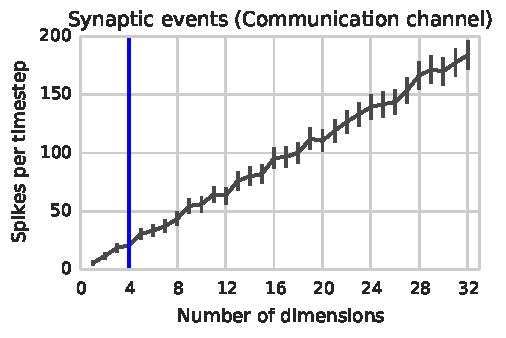
\includegraphics[scale=0.8]{figures/network-1}
    \caption{Spike rates for the pre-synaptic population of a communication channel.  The vertical line indicates the point at which \num{5000} synaptic events per core has been passed. Each population had 70 neurons per dimension.}
    \label{fig:results/network-utilisation}
  \end{figure}

  \section{Exploiting features of the NEF for effective simulation on SpiNNaker}
  \label{sec:exploiting}
  In this section we review an alternative simulation scheme that will meet the constraints of the SpiNNaker hardware for a large range of networks constructed using the NEF.
  % The NEF permits us two different views of the activity of a neural population: that of spikes and that of a set of time-varying vectors.
  % In our simulation scheme we use the second of these to facilitate communication of neural activity between processing cores.
  The details of the NEF described above suggest this alternate, more efficient, implementation for SpiNNaker.
  We note that the synaptic weight matrices are computed via (\ref{eq:weights}).
  This means that all the synaptic weight matrices are exactly \textit{factorable}.
  Moreover every set of connection weights coming into an ensemble will have the same $\alpha_j \vec{e}_j$ factor applied to it.
  We can thus \textit{split} the synaptic connection weight matrices into two parts: the ``encoder'' $\alpha_j \vec{e}_j$ and the ``decoder'' $\vec{d}_i$.
  These matrices are of size $N \times D$ and $D \times N$, where $D$ is the ``dimensionality'' of the representation and is generally much smaller than $N$, the number of neurons.
  We can store the encoder in the core that is simulating the post-synaptic population, and we can store the decoder with the pre-synaptic population.
  This saves significant memory since the two factors are much smaller than the original weight matrix and we only need to store one encoder no matter how many sets of input connections there are.
  However, since the connection weight matrix is split in this way, we can no longer send a packet to represent each spike.
  Rather, the spikes are multiplied by the decoder and the resulting vector value is transmitted.
  Importantly, since the original weight matrices are perfectly factorable, the result is identical to the original SpiNNaker approach in terms of the neural behaviour, but with significantly reduced memory requirements, and, as we shall show, improved processor utilisation.
  \figurename~\ref{fig:algorithm/spikes} illustrates the scheme with the full weight matrix stored in the memory of the post-synaptic core and \figurename~\ref{fig:algorithm/values} illustrates the proposed scheme with the factored matrix split across the pre- and post-synaptic cores and with ``value''-packets being transmitted between the processors.

  \begin{figure*}
    \subfloat[Spike-based transmission]{%
      \label{fig:algorithm/spikes}
      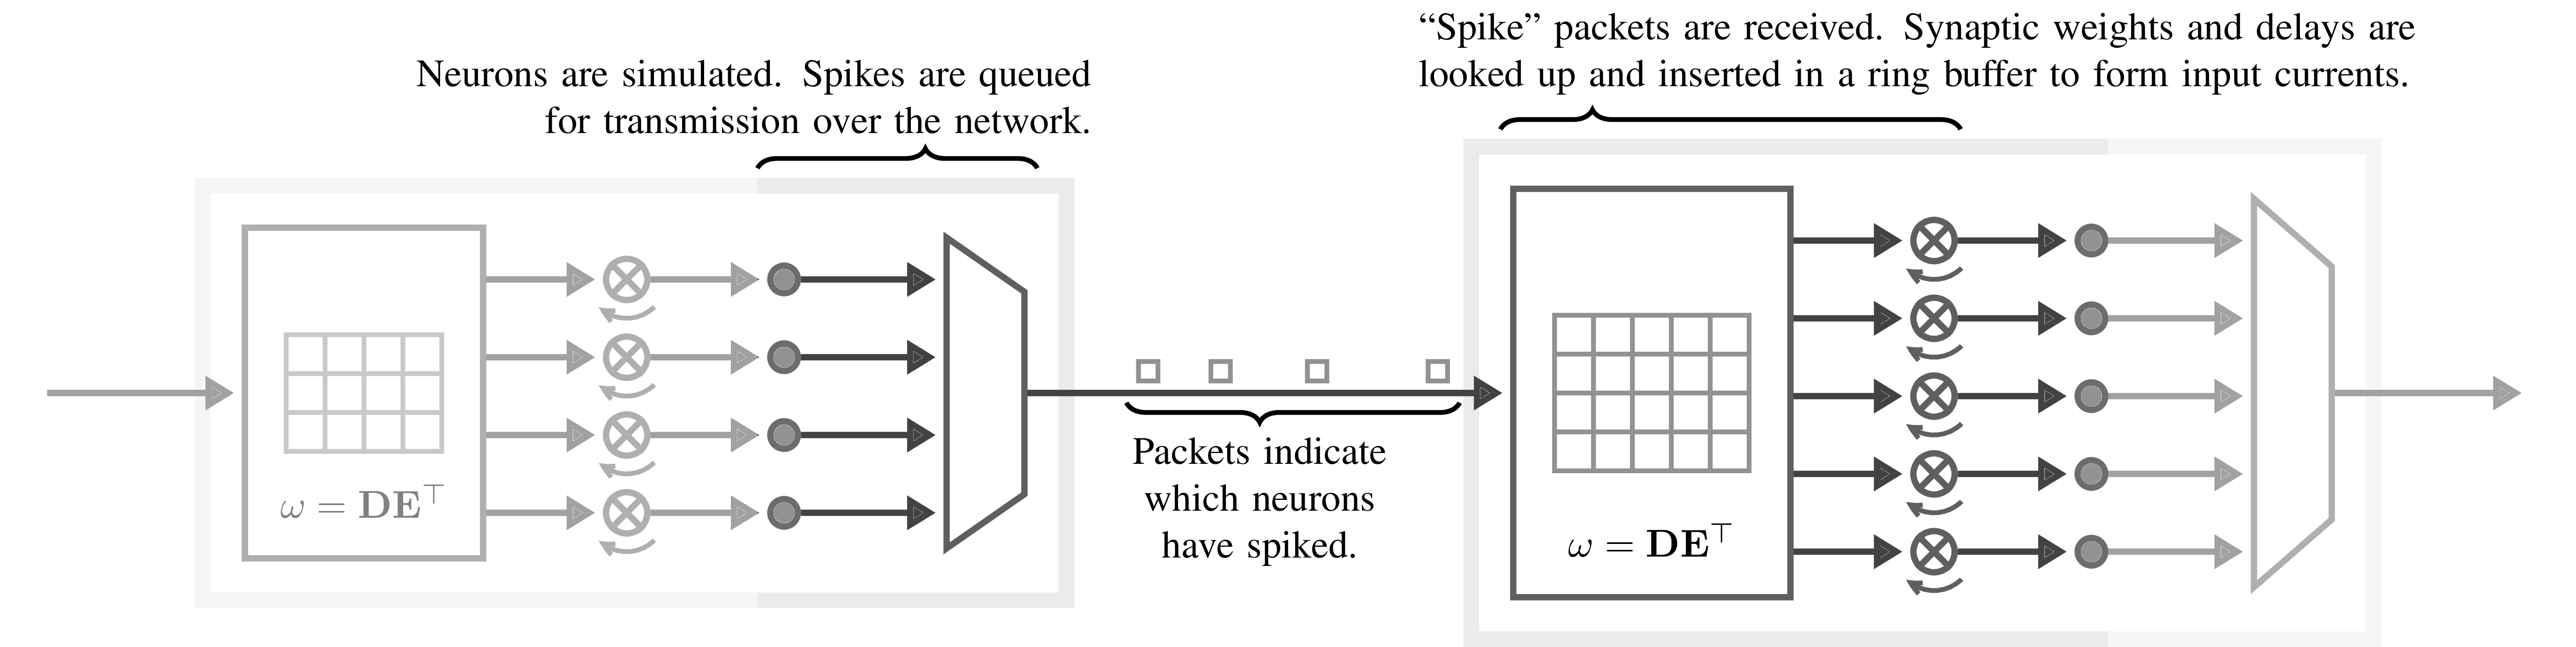
\includegraphics[width=\textwidth]{figures/algorithm_diagram-1}}\\
    \subfloat[Value-based transmission]{%
      \label{fig:algorithm/values}
      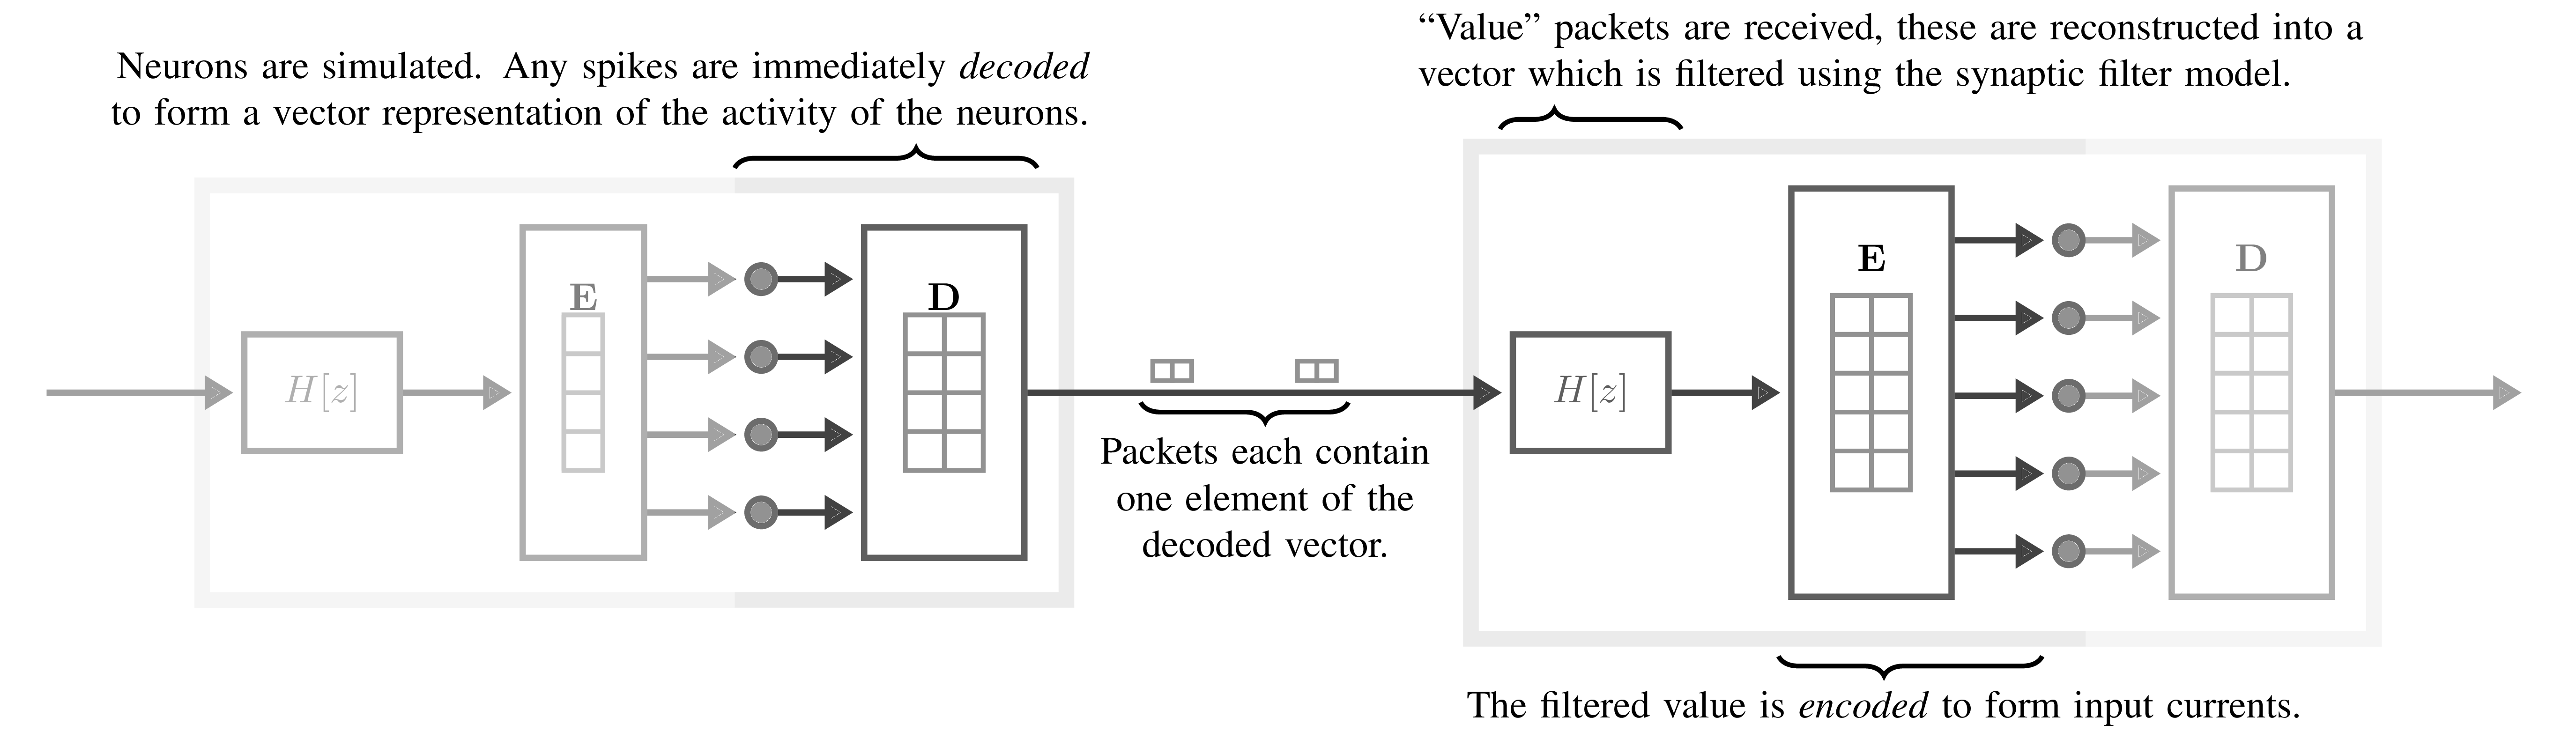
\includegraphics[width=\textwidth]{figures/algorithm_diagram-0}}
      \caption{A comparison of the (a) spike-based and the (b) proposed value-based algorithms.}
  \end{figure*}


  We split the execution time of a processing core into three steps: \textit{input filtering}, \textit{neuron update} and \textit{output}.
  In the ``spike'' simulation scheme the ``inputs'' to a processing core take the form of ``spike'' packets which are used to drive a pipeline that retrieves synaptic weights from SDRAM; in our proposed scheme the inputs take the form of a set of packets whose payloads can be combined to form a vector.
  For example, the processing core simulating population $B$ from \figurename~\ref{fig:background/comms-channel} will receive two packets per time-step from each of the two cores simulating population $A$ which, combined, will form a 2-D vector representing the current decoding of the activity of $A$.
  At the start of each simulation step the reconstructed vector is filtered using the appropriate synaptic filter model to provide the input current to the population -- this is the \textit{input filtering} step.

  During the \textit{neuron update} step the state of each neuron is updated in turn.
  First the input for the neuron is computed by calculating the dot product between the encoding vector for the neuron and the current input to the population ($\alpha_i \vec{e}_i \cdot \vec{x} + J^{bias}_i$ from (\ref{eq:encoding})).
  Then the neuron itself is simulated, for example using the Euler method to compute the next state of a LIF neuron.
  If, during this process, a neuron spikes then its decoding vector ($\vec{d}_i$) is looked up and added to a buffer containing the current decoding of the population activity (as in (\ref{eq:decoding})).
  Once all the neurons have been simulated the output buffer will contain a vector which represents the weighted decoding of any spikes which occurred during the simulation step.

  During the \textit{output} stage each element of the vector contained in the output buffer is transmitted in the payload of a multicast packet whose key uniquely identifies the population and element index.
  The communication fabric routes these ``value'' packets to cores which simulate connected populations of neurons.

  Some ensembles may have multiple outgoing connections with different transformations or functions, meaning that there are multiple decoder matrices to apply when decoding the activity of the population.
  In these cases we combine the matrices such that the decoding vector for any neuron is the concatenation of the required decoders
  (i.e., $\vec{d}_i = \left[\vec{d}_i^{f(\vec{x})},\,\vec{d}_i^{g(\vec{x})},\,\ldots \right]$).

  \section{Results}
  \label{sec:results}

  \subsection{Processor utilisation}
To measure the CPU load when running the algorithm described in \S\ref{sec:exploiting} on SpiNNaker, we developed a simple tool to profile SpiNNaker executables.
In this section we use this tool to analyse how the load on the processors simulating the ensembles in the communication channel network shown in \figurename~\ref{fig:background/comms-channel} varies with number of dimensions and neurons.
\figurename~\ref{fig:results/comm-channel-cpu} shows how the proportion of CPU time spent in the different phases of the algorithm outlined in \S\ref{sec:exploiting} varies with both dimensionality and neuron count.

The \textit{input filtering} and \textit{output} phases of the algorithm both transmit and receive one packet per simulation time-step for every dimension.
Thus the CPU time spent in both phases is predominantly a function of the number dimensions, $D$.
We built simple models of the CPU cycles spent in these phases by fitting the following linear functions to the profiling data using a minimisation of the mean-squared error:
%
\begin{align}
  \mathrm{c}_\mathrm{input} & = 245 + 43 D \label{eq:profiling_input}\\
  \mathrm{c}_\mathrm{output} & = 100 + 702 D \label{eq:profiling_output}
\end{align}
%
Where $\mathrm{c}_\mathrm{input}$ and $\mathrm{c}_\mathrm{output}$ are measured in cycles, \num{200000} of which are available per \SI{1}{\milli\second} simulation time-step when the processor is running at \SI{200}{\mega\hertz}.
During the \textit{neuron update} phase, the dot product of the $D$-dimensional input vector and the $D$-dimensional encoder vector is computed for each of the $N$ neurons.
Additionally, when a neuron spikes, it is decoded by adding its $D$-dimensional decoding vector to the current output.
Consequently the compute requirement of the \textit{neuron update} stage is a function of the both the dimensionality and the number of neurons.
To model this we again fitted a simple, 1st order, 2-D function to the profiling data by minimising the mean-squared error:
%
\begin{equation}
  \mathrm{c}_\mathrm{neuron} = 188 + 69 N + 13 N D\label{eq:profiling_neuron}
\end{equation}
%
Adding these equations together we can model the total CPU cycle count as:
%
\begin{equation}
  \mathrm{c}_\mathrm{total} = 533 + 745 D + 69 N + 13 N D\label{eq:profiling_total}
\end{equation}
%
By substituting $D=1$ into (\ref{eq:profiling_total}), we can see that the maximum number of neurons that could be supported in the 1-D case is 2423. This matches our experimental findings that our new simulator can simulate over 2000 neurons -- double the SpiNNaker system's architectural target of 1000 \parencite{Furber2007}. 
In order to compare this model with the spike-based communication model discussed in \S\ref{sec:background/assessing}, we can further simplify (\ref{eq:profiling_total}) by substituting $D=\frac{N}{70}$ to reflect Eliasmith's \parencite{eliasmith2013build} analysis:
%
\begin{equation}
  \mathrm{c}_\mathrm{total} = 533 + 80 N + 0.19 N^{2}\label{eq:profiling_total_eliasmith}
\end{equation}
%
Finally, using the CPU cycle estimates for updating neuronal state and processing incoming synaptic events quoted by \textcite{Sharp2013} and the incoming spike rates measured in \S\ref{sec:background/assessing}, we can build a similar model of the CPU cycle count of the standard SpiNNaker simulator:
%
\begin{equation}
  \mathrm{c}_\mathrm{spike-based-total} = 128N + 3 N^{2}\label{eq:profiling_spike_based_total}
\end{equation}
% 
These models show that our implementation requires significantly fewer CPU cycles per neuron than the general purpose SpiNNaker simulator, allowing it to simulate up to 834 neurons per core in this configuration. 
This is more than $3.5 \times$ the 236 neurons per core that the general purpose SpiNNaker simulator can achieve in the same configuration.

%% More exposition here

  \begin{figure*}[!t]
    \centering
    \subfloat[16-D]{
      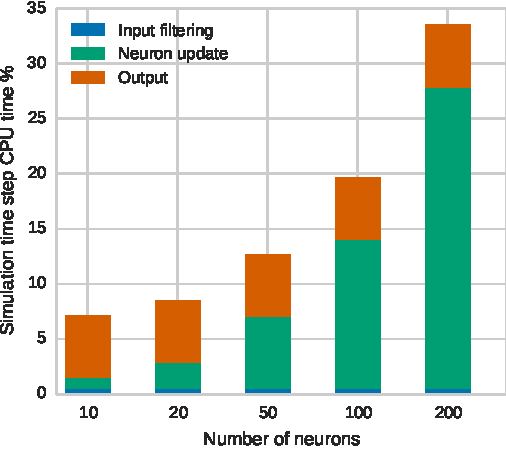
\includegraphics[width=2.5in]{figures/comm_channel_cpu_16d_bar}
    }
    \hfil
    \subfloat[100 neurons per population]{
      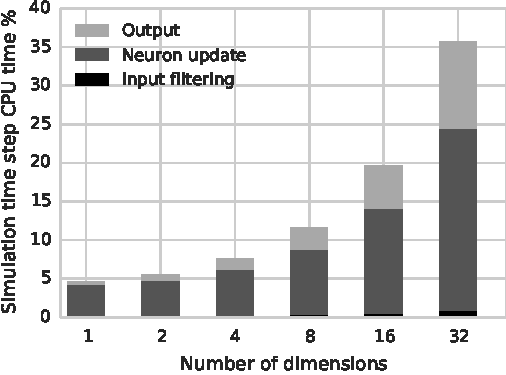
\includegraphics[width=2.5in]{figures/comm_channel_cpu_100n_bar}
    }
    \caption{Mean percentage of 1ms simulation time step spent in different phases of our simulation algorithm when simulating communication channels of varying dimensionality using different numbers of neurons.}
    \label{fig:results/comm-channel-cpu}
  \end{figure*}

  \subsection{Memory utilisation}

  The dense connection weight matrix for any connection between populations of $N_\mathrm{pre}$ and $N_\mathrm{post}$ neurons in the NEF will be of size $N_\mathrm{pre} \times N_\mathrm{post}$ and, under the spike based algorithm, would be stored entirely in the memory of the post-synaptic core.
  When factored weight matrices are substituted for the full weight matrix, as described in \S\ref{sec:exploiting}, the memory usage is split between the pre- and post-synaptic cores.
  The post-synaptic core needs to store a single encoder matrix of size $D_\mathrm{post} \times N_\mathrm{post}$ while the pre-synaptic core will store a decoder matrix of size $D_\mathrm{pre} \times N_\mathrm{pre}$, where $D_\mathrm{population}$ is the dimensionality of the population.

  For example, a 16-D communication channel constructed from two \num{1120}-neuron populations will require \num{1254400} values to be stored in the memory of the post-synaptic core to represent the full weight matrix.
  If factored weight matrices are used then both the pre- and post-synaptic cores must store \num{17920} values, although the post-synaptic core will not need to store any more data for any further incoming connections.
  sing \SI{16}{\bit} to store each synaptic value and, as in our implementation, \SI{32}{\bit} to store each encoder/decoder value this becomes \SI{2.4}{\mebi\byte} to store the full weight matrix or \SI{70.0}{\kibi\byte} each to store the encoder and decoder (a total of \SI{140.0}{\kibi\byte}).
  Factored weight matrices achieve a saving~of~\SI{94.3}{\percent}.

  \begin{table}
    \centering
    \caption{Memory Usage of Synaptic Weights in Basal Ganglia Model}  %% Yuck, Title Case
    \label{tab:results/memory-bg70}
    
\begin{tabular}{r S S S S}
  \toprule
    Inputs & {16} & {32} & {64} & {128} \\
  \midrule
    Full weight matrix / \si{\mebi\byte} & 10.77 & 40.67 & 157.91 & 622.07\\
    Factored / \si{\mebi\byte} & 0.18 & 0.63 & 2.37 & 9.18\\
    Reduction / \si{\percent} & 98.35 & 98.45 & 98.50 & 98.52\\
  \bottomrule
\end{tabular}

    \vskip\baselineskip

    \raggedright Memory usage of the synaptic weights (full matrix and factored) for the standard Basal Ganglia implementation from Nengo (70 neurons per input).
  \end{table}

  Table~\ref{tab:results/memory-bg70} shows the memory usage from the connections within the basal ganglia model used in Spaun.
  The reduction in memory usage that results from using factored weight matrices is significant -- indeed, it should be noted that for a basal ganglia accepting \num{128} inputs representing the connection weights would require the SDRAM of three SpiNNaker chips if full weight matrices were used.

  \subsection{Simulating large-scale models}
  \label{sec:spa-sequence}

  To illustrate the correctness of our technique and to provide a comparison between SpiNNaker and the reference NEF implementation (Nengo \parencite{Bekolay2014}), we simulated a larger model based on the basal ganglia model used in Spaun \parencite{Stewart2010}.

  For the purposes of our benchmark, we assigned a 16-D semantic pointer to each basal ganglia input and generated utility values over time by comparing these to a repeating sequence of semantic pointers. A sample of the basal ganglia input and output are shown in \figurename~\ref{fig:results/basal_ganglia}.

  We simulated this model for \SI{10}{\second} using a SpiNNaker machine and the standard NEF implementation on a standard desktop PC (\SI{3}{\giga\hertz} AMD Athlon II X3 445).
  \figurename~\ref{fig:results/spa-wall-clock} shows the time required to perform certain stages of preparing, uploading data to the SpiNNaker machine, executing the model and retrieving data for two scales of model.
  As expected, SpiNNaker is able to perform the simulation in biological real-time and is thus significantly faster than Nengo for this example despite the additional overheads.
  It is likely that as the scale and complexity of models increase the overheads will follow, but this should be less than the expected growth in simulation time on the PC.

  \begin{figure}[!t]
    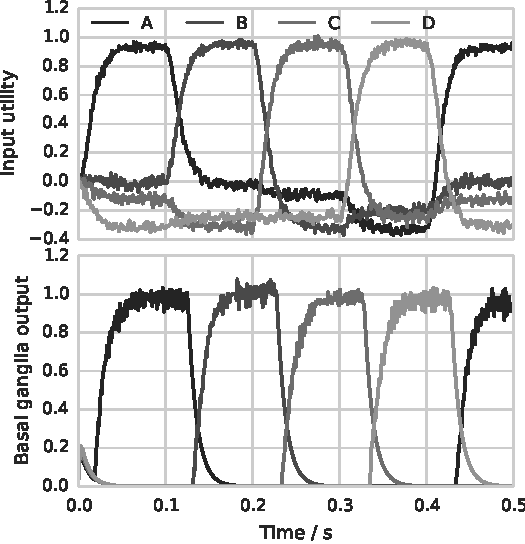
\includegraphics{figures/basal_ganglia}
    \caption{SpiNNaker simulation of the Basal Ganglia model, selecting between 4 inputs labelled $A$, $B$, $C$ and $D$, presented to it in sequence.}
    \label{fig:results/basal_ganglia}
  \end{figure}

  \begin{figure}[!t]
    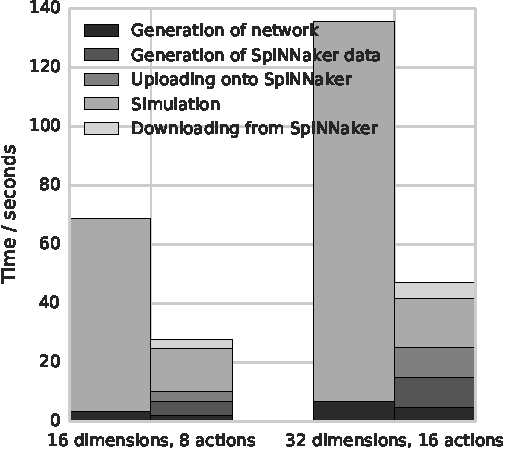
\includegraphics{figures/spa_wall_clock}
    \caption{The time spent in different stages of both the SpiNNaker and the Nengo reference simulators when running the basal ganglia benchmark. }
    \label{fig:results/spa-wall-clock}
  \end{figure}
  \section{Discussion}

  \subsection{Comparison to prior SpiNNaker implementations}

  \textcite{Galluppi2012} demonstrated a SpiNNaker implementation of the NEF using the method described in \S\ref{sec:background/nn}.
  For the reasons advanced in this paper, we believe that it would not have been possible to successfully simulate models of the scale or complexity of Spaun using this system.
  First hand experience with this system indicated that the load time required to transfer full synaptic matrices to a SpiNNaker machine could be extensive. 
To avoid this \citeauthor*{Galluppi2012}\ suggested transmitting factored weight matrices and performing their multiplication on SpiNNaker.
  While this would have reduced the load time it may have resulted in poor accuracy due to the lack of floating point hardware on SpiNNaker.
  Moreover, it would have neither reduced the amount of memory that would be required on SpiNNaker nor reduced the overloading of the processors due to high spike rates and would still have resulted in inefficient use of the architecture.

  \subsection{Comparison to other neuromorphic simulators}

  SpiNNaker is but one of a range of neuromorphic simulators, a family including both analogue (e.g., Neurogrid \parencite{Benjamin2014}, BrainScaleS \parencite{Schemmel2010}) and digital (e.g., TrueNorth \parencite{Merolla2014}) hardware, which aim to reduce the power consumption and execution time for simulating large neural models.
  These simulators can be expected to require less power than SpiNNaker for a given scale of model \parencite{Stromatias2013}, but are limited to simulating the types of neurons and synapses they were fabricated with, whereas SpiNNaker can be reprogrammed to investigate new models.
  In the context of running NEF models of the type discussed in this paper, there is another key limitation of these systems -- the number of hardware synapses associated with each neuron. In the case of TrueNorth, this number is only \num{256} and, for the BrainScaleS architecture, it is \num{16000}, restricting the size of the populations that can be connected using dense connectivity matrices to only 16 and 126 respectively.

  \subsection{Comparison to general purpose computer simulators}

  The reference implementation of the NEF is Nengo \parencite{Bekolay2014}.
  This defines a backend-agnostic set of elements that can be used to construct networks using the principles of the NEF, and a simulation tool which uses the same technique of factoring weight matrices that we have exploited here to reduce memory usage.
  \textcite*{Bekolay2014}\ show that this reference implementation performs well in comparison to alternative PC-based neural simulators such as Brian \parencite{Goodman2009}, NEURON \parencite{carnevale2006neuron} and NEST \parencite{Gewaltig2007}.

  We have extended the work of \citeauthor*{Bekolay2014} by indicating specific reductions in memory usage and by transferring the factored weight matrix simulation scheme to a distributed computing architecture.
  A particular advantage of the SpiNNaker architecture is that it will simulate networks in biological real-time regardless of model scale and complexity (see \figurename~\ref{fig:results/spa-wall-clock}) -- something that is not possible for commodity hardware.
  Furthermore, as a real-time system it is able to interface with neuromorphic hardware (e.g., artificial retinas \parencite{}, or cochleas \parencite{}).

  \subsection{General applicability of the algorithm}

  As SpiNNaker is an example of a message passing architecture we expect that our simulation scheme, transmitting decoded representations of ensemble activity rather than spike activity, to be equally applicable to simulating neural nets on any message passing distributed architecture, such as MPI.

  Additionally, beyond the NEF, factored weight matrices may be applicable to further types of synaptic matrix.
  Furthermore, while we have specifically optimised for the case where the factorisations of all connections terminating at a given population may share the same encoder matrix, this need not be the case.

  \subsection{Future work}

  This work has laid the basis for simulating truly large-scale NEF models in biological real-time.
  We plan several improvements which should enable a greater number of neurons to fit on a single core and, beyond this we anticipate the implementation of further neuron and synapse models.
  In particular, we also intend to better assess the computational cost or gain of value-based transmission when implementing learning rules (e.g., \parencite{Voelker2014}) and investigate how a constant traffic pattern affects the SpiNNaker network architecture.

  \section{Conclusion}

  Some characteristics of neural networks built using the NEF, dense synaptic weight matrices and high firing rates, lead to inefficient use of the SpiNNaker architecture.
  In particular we identified that storing the synaptic matrices for these networks would require large amounts of memory and that the high firing rates and dense neural connectivity would exceed the computational resources available to a SpiNNaker core simulating a model in biological real-time.
  To overcome these constraints we proposed a simulation scheme which used factored weight matrices.
  This proposed scheme requires around 90\% less memory in many cases and is able to simulate many more neurons per core than would otherwise be possible -- in some cases we are able to simulate 2000 neurons per core, double the SpiNNaker architectural target.
  We intend to use the algorithm we have presented to simulate the Spaun functional brain model in biological real-time: a speed-up of 9000 times over commodity hardware.

  \section*{Acknowledgements}

The authors would like to extend their thanks to the organisers of the Telluride Neuromorphic Cognition Engineering Workshop.

  \printbibliography

\end{document}
